%
% 11-bohrmollerup.tex
%
% (c) 2022 Prof Dr Andreas Müller, OST Ostschweizer Fachhochschule
%
\subsection{Der Satz von Bohr-Mollerup
\label{buch:rekursion:subsection:bohr-mollerup}}
\begin{figure}
\centering
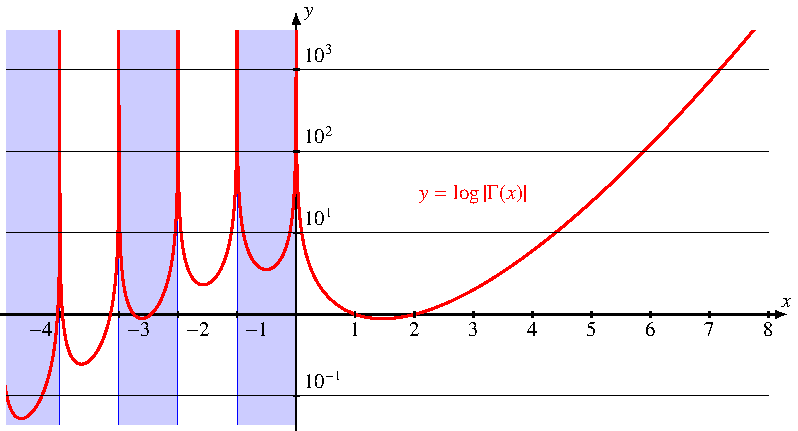
\includegraphics{chapters/040-rekursion/images/loggammaplot.pdf}
\caption{Der Graph der Funktion $\log|\Gamma(x)|$ ist für $x>0$ konvex. 
Die blau hinterlegten Bereiche zeigen an, wo die Gamma-Funktion
negative Werte annimmt.
\label{buch:rekursion:gamma:loggammaplot}}
\end{figure}
Die Integralformel und die Grenzwertdefinition für die Gamma-Funktion
zeigen beide, dass das Problem der Ausdehnung der Fakultät zu einer
Funktion $\mathbb{C}\to\mathbb{C}$ eine Lösung hat, aber es ist noch
nicht klar, in welchem Sinn dies die einzig mögliche Lösung ist.
Der Satz von Bohr-Mollerup gibt darauf eine Antwort.

Der Graph in Abbildung~\ref{buch:rekursion:gamma:loggammaplot}
zeigt, dass die Werte der Gamma-Funktion für $x>0$ so schnell
anwachsen, dass sogar die Funktion $\log|\Gamma(x)|$ konvex ist.
Der Satz von Bohr-Mollerup besagt, dass diese Eigenschaft zur
Charakterisierung der Gamma-Funktion verwendet werden kann.

\begin{satz}
\label{buch:satz:bohr-mollerup}
Eine Funktion $f\colon \mathbb{R}^+\to\mathbb{R}$ mit den Eigenschaften
\begin{enumerate}[i)]
\item $f(1)=1$,
\item $f(x+1)=xf(x)$ für alle $x\in\mathbb{R}^+$ und
\item die Funktion $\log f(t)$ ist konvex
\end{enumerate}
ist die Gamma-Funktion: $f(t)=\Gamma(t)$.
\index{Satz!von Bohr-Mollerup}%
\index{Bohr-Mollerup, Satz von}%
\end{satz}

Für den Beweis verwenden wir die folgende Eigenschaft einer konvexen
Funktion $g(x)$.
Sei
\begin{equation}
S(y,x) = \frac{g(y)-g(x)}{y-x}
\qquad\text{für $y-x$}
\end{equation}
die Steigung der Sekante zwischen den Punkten $(x,g(x))$ und $(y,g(y))$
des Graphen von $g$.
Da $g$ konvex ist, ist $S(y,x)$ eine monoton wachsende Funktion 
der beiden Variablen $x$ und $y$, solange $y>x$.

\begin{proof}[Beweis]
Wir halten zunächst fest, dass die Bedingungen i) und ii) zur Folge haben,
dass $f(n+1)=n!$ ist für alle positiven natürlichen Zahlen.
Für die Steigung einer Sekante der Funktion $g(x)=\log f(x)$ kann damit
für natürliche Argumente bereits berechnet werden, es ist
\[
S(n,n+1)
=
\frac{\log n! - \log (n-1)!}{n+1-n}
=
\frac{\log n + \log (n-1)! - \log(n-1)!}{1}
=
\log n
\]
und entsprechend auch $S(n-1,n) = \log(n-1)$.

\begin{figure}
\begin{center}
\begin{tikzpicture}[>=latex,thick]
\draw (-6,0) -- (6,0);

\node at (-5,0) [above] {$n-1\mathstrut$};
\node at (0,0) [above] {$n\mathstrut$};
\node at (3,0) [above] {$n+x\mathstrut$};
\node at (5,0) [above] {$n+1\mathstrut$};

\node[color=blue] at (-5,-2.3) {$S(n-1,n)\mathstrut$};
\node[color=red] at (-1.666,-2.3) {$S(n-1,n+x)\mathstrut$};
\node[color=darkgreen] at (1.666,-2.3) {$S(n,n+x)\mathstrut$};
\node[color=orange] at (5,-2.3) {$S(n,n+1)\mathstrut$};

\node at (-3.333,-2.3) {$<\mathstrut$};
\node at (0,-2.3) {$<\mathstrut$};
\node at (3.333,-2.3) {$<\mathstrut$};

\draw[color=blue] (-5,0) -- (-5,-2) -- (0,0);
\draw[color=red] (-5,0) -- (-1.666,-2) -- (3,0);
\draw[color=darkgreen] (0,0) -- (1.666,-2) -- (3,0);
\draw[color=orange] (0,0) -- (5,-2) -- (5,0);

\fill (-5,0) circle[radius=0.08];
\fill (0,0) circle[radius=0.08];
\fill (3,0) circle[radius=0.08];
\fill (5,0) circle[radius=0.08];

\draw[double,color=blue] (-5,-2.5) -- (-5,-3.0);
\draw[double,color=orange] (5,-2.5) -- (5,-3.0);

\node[color=blue] at (-5,-3.3) {$\log (n-1)\mathstrut$};
\node[color=orange] at (5,-3.3) {$\log (n)\mathstrut$};

\end{tikzpicture}
\end{center}
\caption{Für den Beweis des Satzes von Bohr-Mollerup wird die
Sekantensteigung $S(x,y)$ für die Argumente $n-1$, $n$, $n+x$ und $n+1$
verwendet.
\label{buch:rekursion:fig:bohr-mollerup}}
\end{figure}
Wir wenden jetzt die eben erwähnte Tatsache, dass $S(x,y)$ monoton
wachsend ist, auf die Punkte $n-1$, $n$, $n+x$ und $n+1$ wie
in Abbildung~\ref{buch:rekursion:fig:bohr-mollerup} an, wobei
$0<x<1$ ist.

Die linke Ungleichung in Abbildung~\ref{buch:rekursion:fig:bohr-mollerup}
ist
\begin{align}
\log(n-1)
&<
S(n-1,n+x)
=
\frac{\log f(n+x) -\log(n-2)!}{n+x-n+1}
\notag
\\
(x+1)\log(n-1) + \log(n-2)!
&< \log f(n+x),
\notag
\\
x\log(n-1) + \log(n-1)!
&< \log f(n+x)
\label{buch:rekursion:bohr-mollerup:eqn1}
\intertext{sie schätzt $\log f(n+x)$ nach unten ab.
Die Exponentialfunktion ist monoton wachsen, wendet man sie auf
\eqref{buch:rekursion:bohr-mollerup:eqn1} an, erhält man}
(n-1)^x (n-1)!
&<
f(n+x).
\label{buch:rekursion:bohr-mollerup:ungllinks}
\end{align}
Ganz ähnlich folgt aus der Ungleichung rechts in
Abbildung~\ref{buch:rekursion:fig:bohr-mollerup}
\begin{align}
\frac{\log f(n+x)-\log (n-1)!}{n+x-n}
&< \log n
\notag
\\
\log f(n+x) - \log(n-1)!
&<
x \log n
\notag
\\
\log f(n+x) 
&<
x\log n + \log(n-1)!
\notag
\intertext{und nach Anwendung der Exponentialfunktion}
f(n+x)
&<
n^x (n-1)!
\label{buch:rekursion:bohr-mollerup:unglrechts}
\end{align}
Die Funktion $f(n+x)$ können wir jetzt mit der Funktionalgleichung ii)
durch $f(x)$ ausdrücken:
\begin{align*}
f(n+x)
&=
(x+n-1)f(n+x-1)
\\
&=
(x+n-1)(x+n-2)f(n+x-2)
\\
&\vdots
\\
&=
(x+n-1)(x+n-2)\dots x\,f(x)
=
(x)_n f(x).
\end{align*}
Zusammen mit den Ungleichungen
\eqref{buch:rekursion:bohr-mollerup:ungllinks}
und
\eqref{buch:rekursion:bohr-mollerup:unglrechts}
erhalten wir
\begin{align*}
(n-1)^x (n-1)!
&<
(x)_n f(x)
<
n^x (n-1)!
\intertext{oder nach Division durch $(x)_n$}
%\underbrace{
\frac{(n-1)^x (n-1)!}{(x)_n}
%}_{\displaystyle\to \Gamma(x)}
&< f(x)
<
\frac{n^x (n-1)!}{(x)_n}
=
%\underbrace{
\frac{n^x n!}{(x)_{n+1}}
%}_{\displaystyle\to \Gamma(x)}
\cdot
%\underbrace{
\frac{x+n}{n}
%}_{\displaystyle\to 1}
.
\end{align*}
Der Ausdruck ganz links und der erste Bruch rechts konvergieren
für $n\to\infty$ beide gegen $\Gamma(x)$ und der Bruch ganz rechts
konvergiert gegen $1$.
Daher muss auch $f(x)=\Gamma(x)$ sein.
\end{proof}
